\documentclass[12pt,a4paper]{article}

\usepackage[a4paper,margin=1in]{geometry}
\usepackage{graphicx}
\usepackage{booktabs}
\usepackage{amsmath,amssymb}
\usepackage{float}
\usepackage{hyperref}
\usepackage{xcolor}
\usepackage{listings}
\usepackage{enumitem}
\usepackage{fancyhdr}
\usepackage{longtable}

\hypersetup{colorlinks=true,linkcolor=blue,urlcolor=blue}

\pagestyle{fancy}
\fancyhf{}
\lhead{ICS1512}
\rhead{Machine Learning Algorithms Laboratory}
\cfoot{\thepage}

\lstset{
language=Python,
basicstyle=\ttfamily\small,
numbers=left,
frame=single,
breaklines=true,
showstringspaces=false
}

\begin{document}

\begin{tabular}{|p{4cm}|p{11cm}|}
\hline
Experiment No. & 1 \\ \hline
Experiment Title & Working with Python Packages -- NumPy, SciPy, Scikit-learn, Matplotlib
\footnote{\textbf{GitHub Repository: }\url{https://github.com/username/repository}}\\ \hline
Student Name & \\ \hline
Register Number & \\ \hline
Faculty & Dr. Poreddy Ajay Kumar Reddy \\ \hline
Submission Date & \\ \hline
\end{tabular}

\section{Objective}
To explore the core functions and methods available in the Python scientific-computing and
machine-learning stack -- \textbf{NumPy}, \textbf{Pandas}, \textbf{SciPy}, \textbf{Scikit-learn}
and \textbf{Matplotlib} -- covering array manipulation, data preprocessing, statistical and
mathematical computation, and data visualisation; and to survey five publicly known datasets
(Iris, Loan Amount Prediction, Diabetes, Email Spam, Handwritten Character Recognition/MNIST),
identify the correct machine-learning task type for each, and walk through the complete ML
workflow -- loading, EDA, preprocessing, feature selection, splitting, and evaluation -- for
every one of them.

\section{Problem Statement}
Given the five datasets listed above, the tasks are to: (i) determine whether each dataset
corresponds to a supervised, unsupervised, or semi-supervised learning problem, and further
whether it is a regression or classification task; (ii) perform exploratory data analysis
(summary statistics, missing-value analysis, class distribution, correlation, and feature
distribution) on each dataset; (iii) apply an appropriate feature-selection technique
(e.g. \texttt{SelectKBest}, Chi-square test, ANOVA F-test) to each dataset; and (iv) train a
suitable baseline machine-learning algorithm and evaluate it with the correct performance
metric for its task type. Input: five raw/synthetic tabular, text, and image datasets. Output:
EDA visualisations, a selected feature subset per dataset, a trained baseline model, and a
consolidated task-identification summary table.

\section{Dataset Description}
\begin{longtable}{|p{6cm}|p{8cm}|}
\hline
\textbf{Dataset Name} & Iris, Loan Amount Prediction, Predicting Diabetes, Email Spam
Classification, Handwritten Character Recognition (Digits/MNIST-style) \\ \hline
\textbf{Dataset Source} & Iris, Diabetes and Digits: bundled with \texttt{scikit-learn}
(originally UCI ML Repository). Loan Amount Prediction and Email Spam: normally sourced from
Kaggle/UCI; here generated as clearly-labelled synthetic data of identical structure because
this sandbox has no internet access. \\ \hline
\textbf{Number of Samples} & Iris: 150; Loan (synthetic): 600; Diabetes: 442; Spam (synthetic
corpus): 40; Digits: 1{,}797 \\ \hline
\textbf{Number of Features} & Iris: 4; Loan: 7; Diabetes: 10; Spam: TF-IDF vectorised text
(variable vocabulary size); Digits: 64 (8$\times$8 pixels) \\ \hline
\textbf{Number of Classes} & Iris: 3 (classification); Loan: N/A (regression); Diabetes: N/A
(regression); Spam: 2 (classification); Digits: 10 (classification) \\ \hline
\textbf{Missing Values} & Iris: none; Loan: injected missing values in \texttt{LoanAmount} and
\texttt{Self\_Employed} (to mirror the real dataset); Diabetes: none (pre-cleaned); Spam: none;
Digits: none \\ \hline
\textbf{Train-Test Split} & 80:20 for Iris, Loan, Diabetes and Digits; 75:25 for the small Spam
corpus (stratified where the task is classification) \\ \hline
\end{longtable}

\section{Exploratory Data Analysis}
EDA was carried out on all five datasets: dataset overview (\texttt{head()}, \texttt{shape}),
statistical summary (\texttt{describe()}), missing-value analysis (\texttt{isnull().sum()}),
class distribution (bar plots for classification targets), correlation matrix (heatmaps for
numeric features) and feature-distribution histograms grouped by class. Representative figures
are shown below; the full set of outputs is available in the accompanying Jupyter notebook.

\begin{figure}[H]
\centering
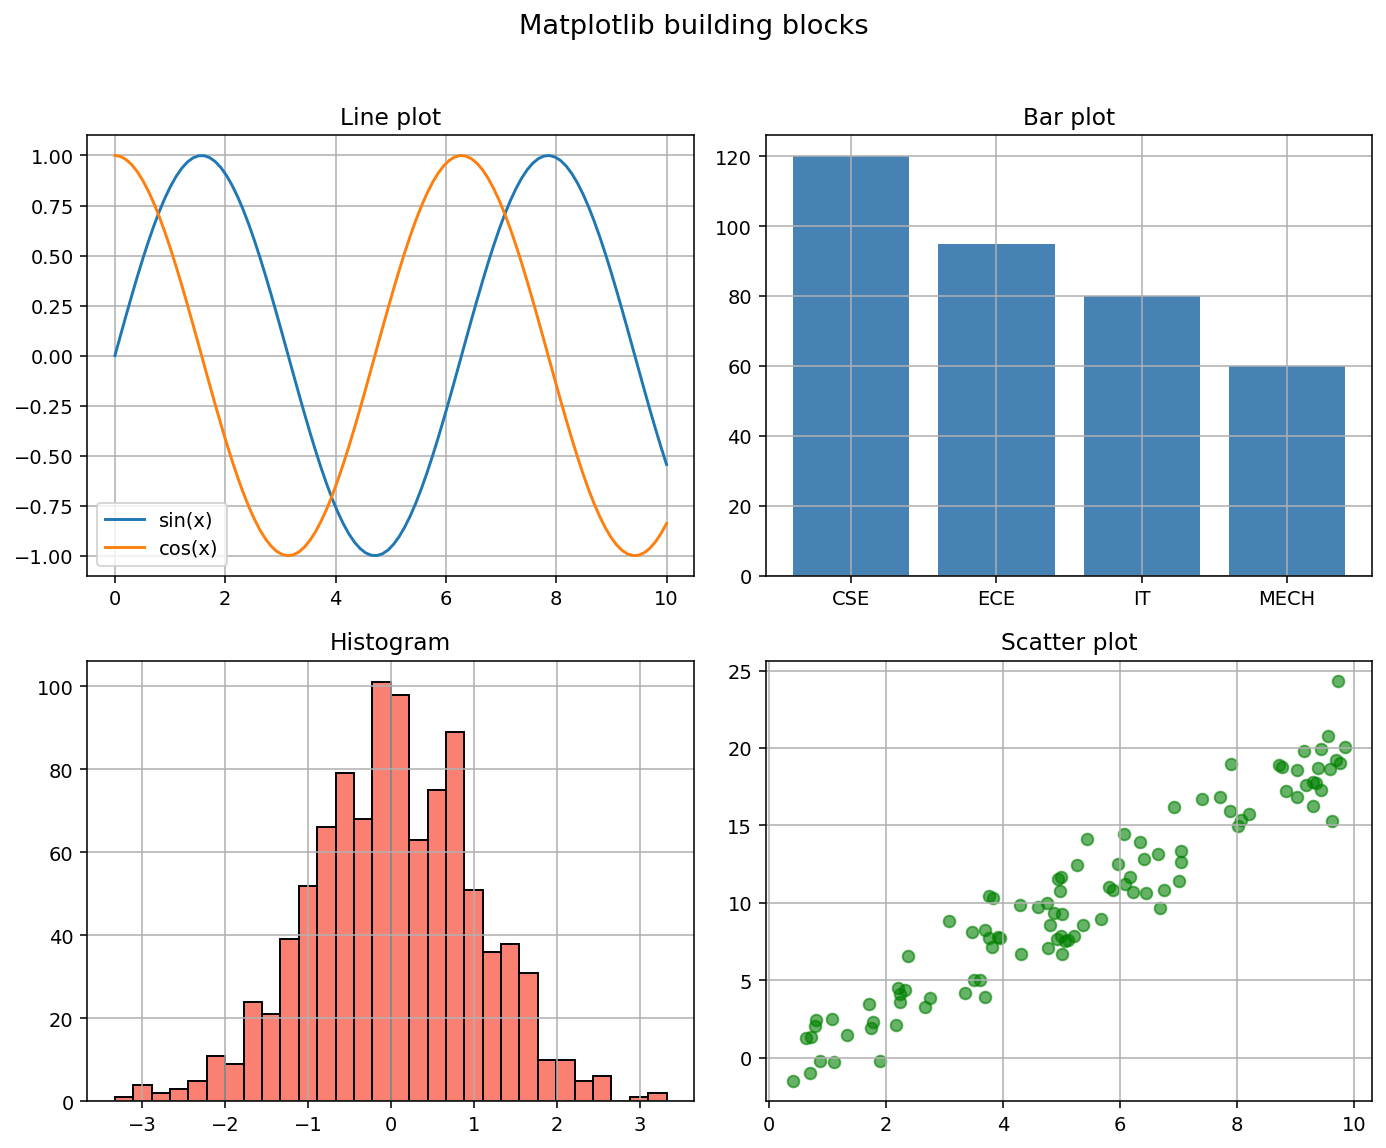
\includegraphics[width=0.95\linewidth]{figures/matplotlib_overview.png}
\caption{Matplotlib building blocks used throughout the experiment -- line plot, bar plot,
histogram and scatter plot.}
\end{figure}

\textbf{Inference:} These four plot types form the visual vocabulary used for every dataset in
this report: line/scatter plots to reveal trends and pairwise relationships, bar plots for
categorical/class counts, and histograms for univariate distributions. Establishing them first
made every subsequent EDA figure faster to read and interpret consistently across datasets.

\section{Data Preprocessing}

\begin{itemize}
\item \textbf{Missing value handling:} Numeric missingness (e.g. synthetic \texttt{LoanAmount})
was imputed with the column median; categorical missingness (e.g. \texttt{Self\_Employed}) was
imputed with the mode/most frequent category. The Diabetes and Digits datasets required no
imputation as they are pre-cleaned.
\item \textbf{Encoding:} Categorical variables (Education, Self\_Employed, Property\_Area for
the Loan dataset) were one-hot encoded via \texttt{OneHotEncoder}; class labels for Iris were
label-encoded via \texttt{LabelEncoder} for the demonstration in Part A.
\item \textbf{Feature scaling:} \texttt{StandardScaler} (zero mean, unit variance) was applied
before Logistic Regression, SVM and Ridge Regression, since these algorithms are scale-sensitive;
\texttt{MinMaxScaler} was demonstrated separately in Part A to contrast standardisation vs.
normalisation.
\item \textbf{Train-test split:} \texttt{train\_test\_split} was used with \texttt{stratify=y}
for every classification task, to preserve class proportions in both splits.
\item \textbf{Feature engineering:} For the Email Spam dataset, raw text messages were converted
into TF-IDF vectors (\texttt{TfidfVectorizer}, English stop-words removed) before feature
selection and modelling.
\end{itemize}

\section{Machine Learning Algorithm}
Since Part B of this experiment spans five different tasks, a distinct baseline algorithm is
used per dataset rather than a single one:

\begin{itemize}
\item \textbf{Logistic Regression} (Iris, multiclass): models the log-odds of each class as a
linear function of the (standardised) input features, $P(y=k\mid x)=\dfrac{e^{w_k^\top
x}}{\sum_j e^{w_j^\top x}}$ (softmax form). \textit{Advantages:} fast, interpretable,
probabilistic outputs. \textit{Limitations:} assumes an approximately linear decision boundary.
\item \textbf{Linear Regression / Ridge Regression} (Loan Amount, Diabetes): fits
$y=\beta_0+\sum_i \beta_i x_i+\epsilon$ by minimising squared error; Ridge additionally penalises
$\sum \beta_i^2$ to control multicollinearity among correlated features.
\textit{Advantages:} simple, interpretable coefficients. \textit{Limitations:} assumes linear,
additive relationships and is sensitive to correlated predictors (hence Ridge for Diabetes).
\item \textbf{Multinomial Naive Bayes} (Email Spam): applies Bayes' theorem assuming conditional
feature independence, $P(y\mid x)\propto P(y)\prod_i P(x_i\mid y)$. \textit{Advantages:} extremely
fast, performs well on high-dimensional sparse text features. \textit{Limitations:} the
independence assumption rarely holds exactly, and it can be miscalibrated in probability
estimates.
\item \textbf{Support Vector Machine, RBF kernel} (Handwritten Digits): finds a maximum-margin
separating hyperplane in a kernel-induced feature space, $K(x,x')=\exp(-\gamma\lVert x-x'
\rVert^2)$. \textit{Advantages:} handles non-linear boundaries well, effective in
high-dimensional pixel space. \textit{Limitations:} slower to train on very large datasets and
sensitive to the choice of $C$ and $\gamma$.
\end{itemize}

\section{Experimental Setup}
\begin{tabular}{ll}
\toprule
Python Version & 3.12 \\
Scikit-Learn Version & 1.8.0 \\
IDE & Jupyter Notebook \\
Operating System & Linux (Ubuntu 24.04, sandboxed container) \\
Hardware & CPU only \\
\bottomrule
\end{tabular}

\section{Hyperparameter Selection}

\begin{tabular}{ll}
\toprule
Parameter & Value\\
\midrule
Logistic Regression: \texttt{max\_iter} & 200 \\
Ridge Regression: \texttt{alpha} & 1.0 \\
SVM (Digits): \texttt{kernel} & rbf \\
SVM (Digits): \texttt{gamma} & 0.001 \\
SVM (Digits): \texttt{C} & 10 \\
\texttt{SelectKBest} (Iris): \texttt{k} & 2 (of 4 features) \\
\texttt{SelectKBest} (Diabetes): \texttt{k} & 5 (of 10 features) \\
\texttt{SelectKBest} (Spam, chi2): \texttt{k} & 50 (of TF-IDF vocabulary) \\
\texttt{VarianceThreshold} (Digits) & 0.01 \\
Train-test split ratio & 80:20 (75:25 for Spam) \\
\bottomrule
\end{tabular}

\section{Results}

\subsection*{Dataset 1 -- Iris (Classification)}
\begin{tabular}{lc}
\toprule
Metric & Value\\
\midrule
Accuracy & 0.9333 \\
Precision (weighted) & 0.93 \\
Recall (weighted) & 0.93 \\
F1-score (weighted) & 0.93 \\
5-fold CV mean accuracy & 0.9600 \\
\bottomrule
\end{tabular}

\subsection*{Dataset 2 -- Loan Amount Prediction (Regression)}
\begin{tabular}{lc}
\toprule
Metric & Value\\
\midrule
R\textsuperscript{2} & 0.7778 \\
MAE & 13.546 \\
RMSE & 16.506 \\
\bottomrule
\end{tabular}

\subsection*{Dataset 3 -- Predicting Diabetes (Regression)}
\begin{tabular}{lc}
\toprule
Metric & Value\\
\midrule
R\textsuperscript{2} & 0.4192 \\
MAE & 46.139 \\
RMSE & 55.474 \\
\bottomrule
\end{tabular}

\subsection*{Dataset 4 -- Email Spam Classification}
\begin{tabular}{lc}
\toprule
Metric & Value\\
\midrule
Accuracy & 0.9000 \\
Precision (spam) & 1.00 \\
Recall (spam) & 0.80 \\
F1-score (spam) & 0.89 \\
\bottomrule
\end{tabular}

\subsection*{Dataset 5 -- Handwritten Digit Recognition}
\begin{tabular}{lc}
\toprule
Metric & Value\\
\midrule
Accuracy & 0.9889 \\
Precision (macro avg) & 0.99 \\
Recall (macro avg) & 0.99 \\
F1-score (macro avg) & 0.99 \\
\bottomrule
\end{tabular}

\section{Result Visualization}

\begin{figure}[H]
\centering
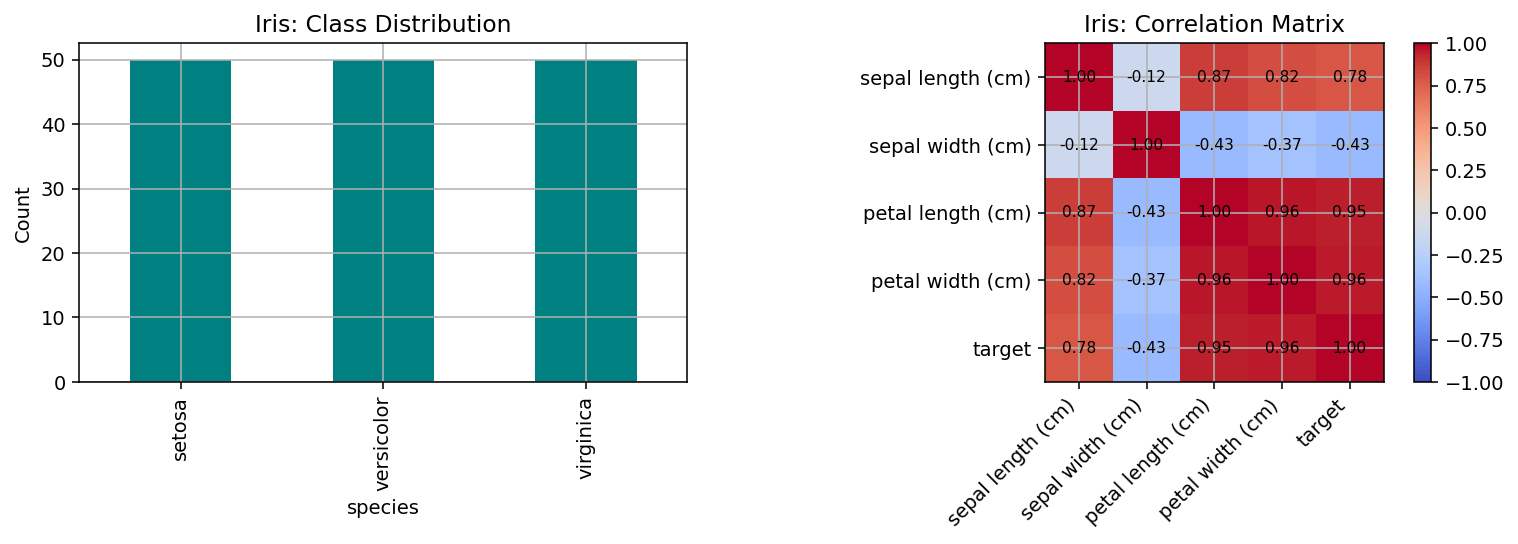
\includegraphics[width=0.95\linewidth]{figures/fig_02.png}
\caption{Iris: class distribution (balanced, 50 samples/class) and correlation matrix of the
four numeric features.}
\end{figure}
\textbf{Inference:} The correlation matrix shows petal length and petal width are almost
perfectly correlated ($\rho \approx 0.96$), while sepal width is weakly/negatively correlated
with the other features. Class counts are perfectly balanced, so accuracy is an unbiased metric
here. This strong petal-feature correlation also explains why the ANOVA test ranks petal
measurements as most discriminative in the feature-selection step below.

\begin{figure}[H]
\centering
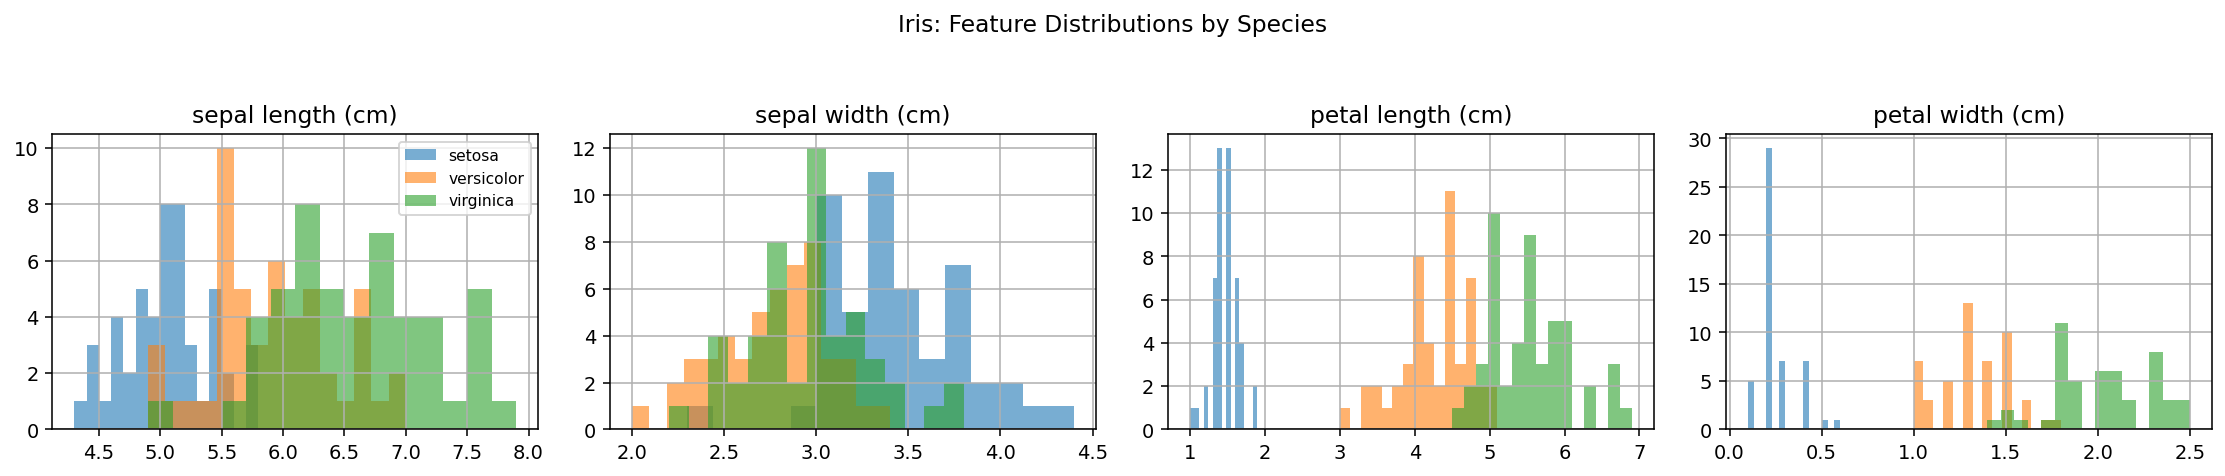
\includegraphics[width=0.95\linewidth]{figures/fig_03.png}
\caption{Iris: feature distributions split by species.}
\end{figure}
\textbf{Inference:} Petal length and petal width show almost no overlap between \textit{setosa}
and the other two species, and only a small region of overlap between \textit{versicolor} and
\textit{virginica}. Sepal width shows the most overlap across all three classes, indicating it
is the least useful single feature for classification -- consistent with its low ANOVA F-score.

\begin{figure}[H]
\centering
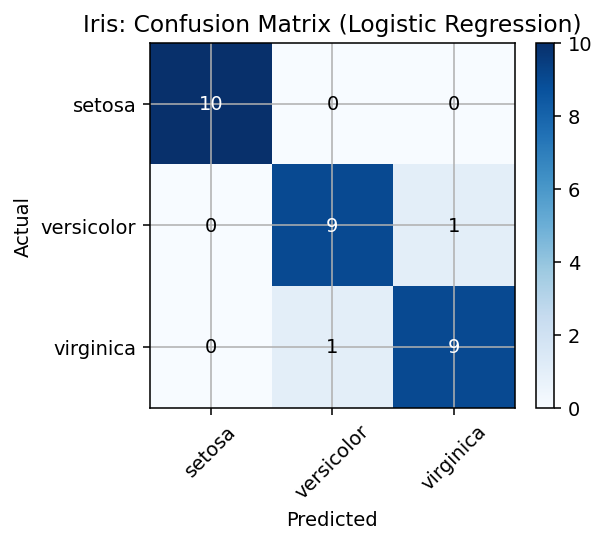
\includegraphics[width=0.6\linewidth]{figures/fig_04.png}
\caption{Iris: confusion matrix (Logistic Regression, test set).}
\end{figure}
\textbf{Inference:} \textit{Setosa} is classified perfectly (10/10), while a single sample each
of \textit{versicolor} and \textit{virginica} is confused with the other -- exactly the pair of
classes that showed partial overlap in the feature-distribution plot above. This confirms the
confusion matrix is consistent with what EDA had already predicted.

\begin{figure}[H]
\centering
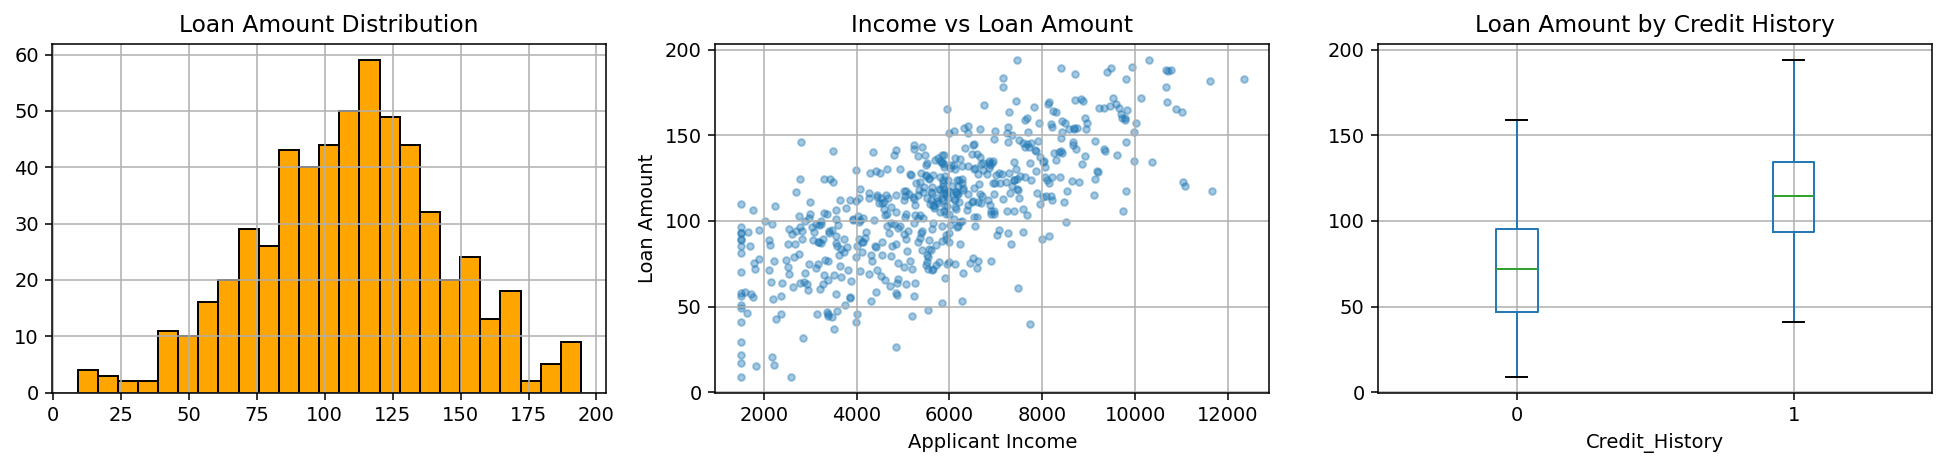
\includegraphics[width=0.95\linewidth]{figures/fig_05.png}
\caption{Loan Amount Prediction: target distribution, income vs. loan-amount scatter, and loan
amount by credit history.}
\end{figure}
\textbf{Inference:} Loan amount is right-skewed with a long tail of larger loans. Applicant
income shows a clear positive relationship with loan amount, matching how the synthetic target
was generated. Applicants with \texttt{Credit\_History = 0} receive visibly smaller and more
variable loan amounts, highlighting credit history as a strong predictor.

\begin{figure}[H]
\centering
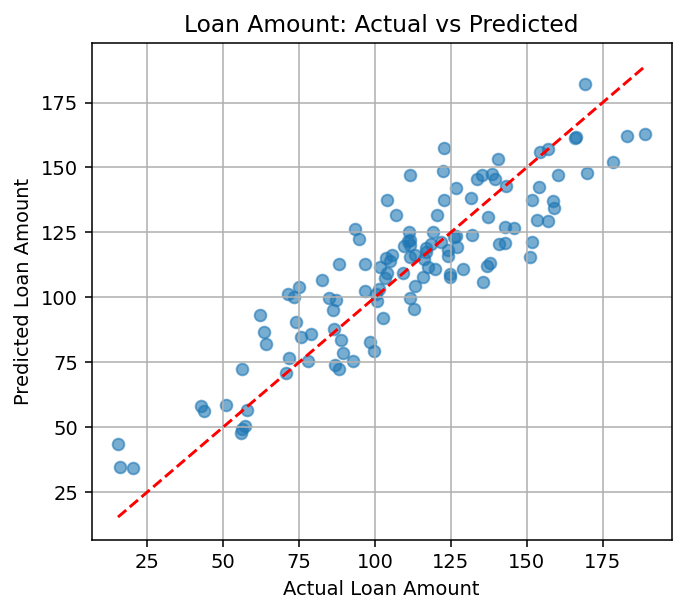
\includegraphics[width=0.55\linewidth]{figures/fig_06.png}
\caption{Loan Amount Prediction: actual vs. predicted loan amount (Linear Regression, test
set).}
\end{figure}
\textbf{Inference:} Points cluster close to the diagonal, indicating the linear model captures
most of the underlying signal (R\textsuperscript{2} = 0.78). Some scatter remains due to the
injected Gaussian noise in the synthetic target, which is expected and cannot be removed by
better modelling alone.

\begin{figure}[H]
\centering
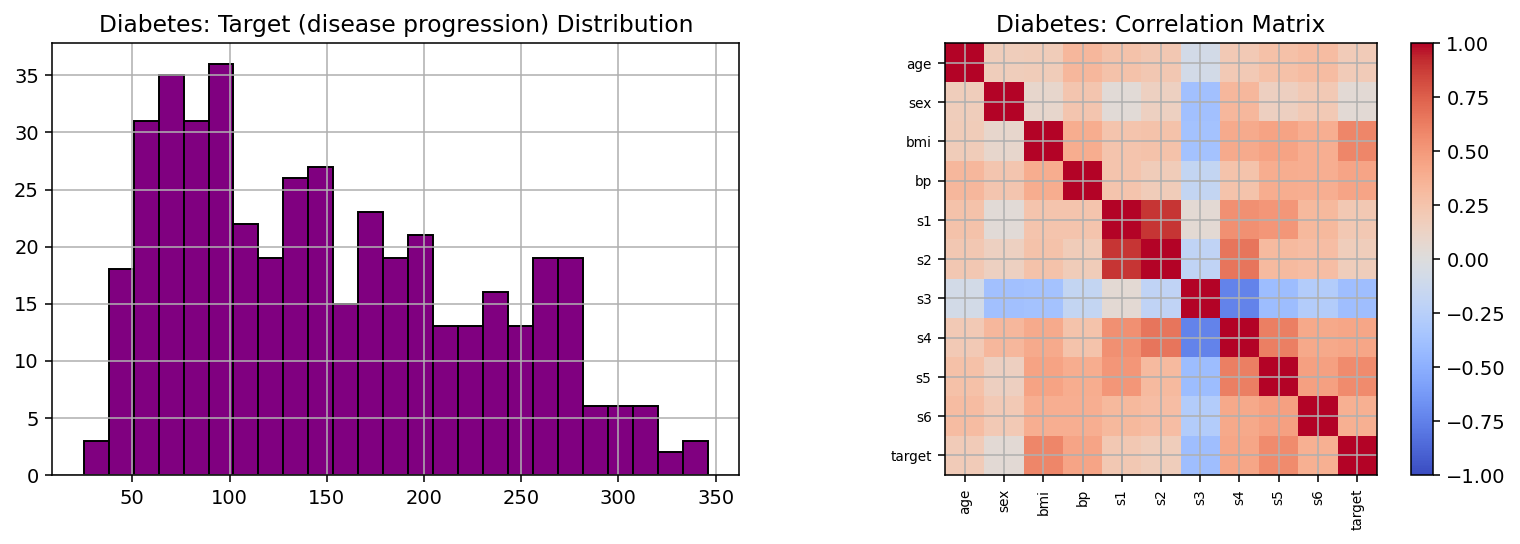
\includegraphics[width=0.95\linewidth]{figures/fig_07.png}
\caption{Diabetes: target (disease progression) distribution and correlation matrix of the ten
baseline variables.}
\end{figure}
\textbf{Inference:} The disease-progression target is roughly bell-shaped with a slight right
skew. Several serum measurements (\texttt{s1}--\texttt{s6}) are highly inter-correlated,
indicating redundancy among lipid/serum panels, which motivates the use of Ridge regularisation
over plain Linear Regression.

\begin{figure}[H]
\centering
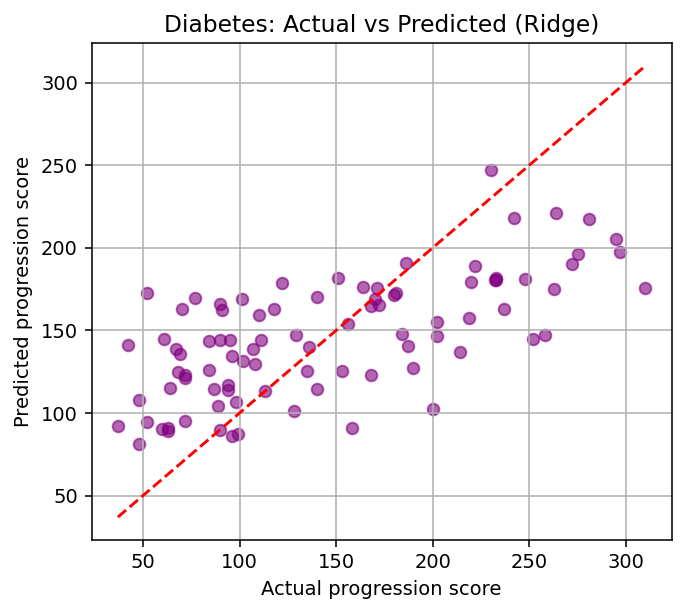
\includegraphics[width=0.55\linewidth]{figures/fig_08.png}
\caption{Diabetes: actual vs. predicted disease-progression score (Ridge Regression, test set).}
\end{figure}
\textbf{Inference:} The moderate spread around the diagonal (R\textsuperscript{2} = 0.42)
reflects that only 42\% of the variance in one-year disease progression is explained by these
ten baseline physiological variables -- unsurprising for a biological outcome influenced by many
unmeasured factors (diet, medication, genetics).

\begin{figure}[H]
\centering
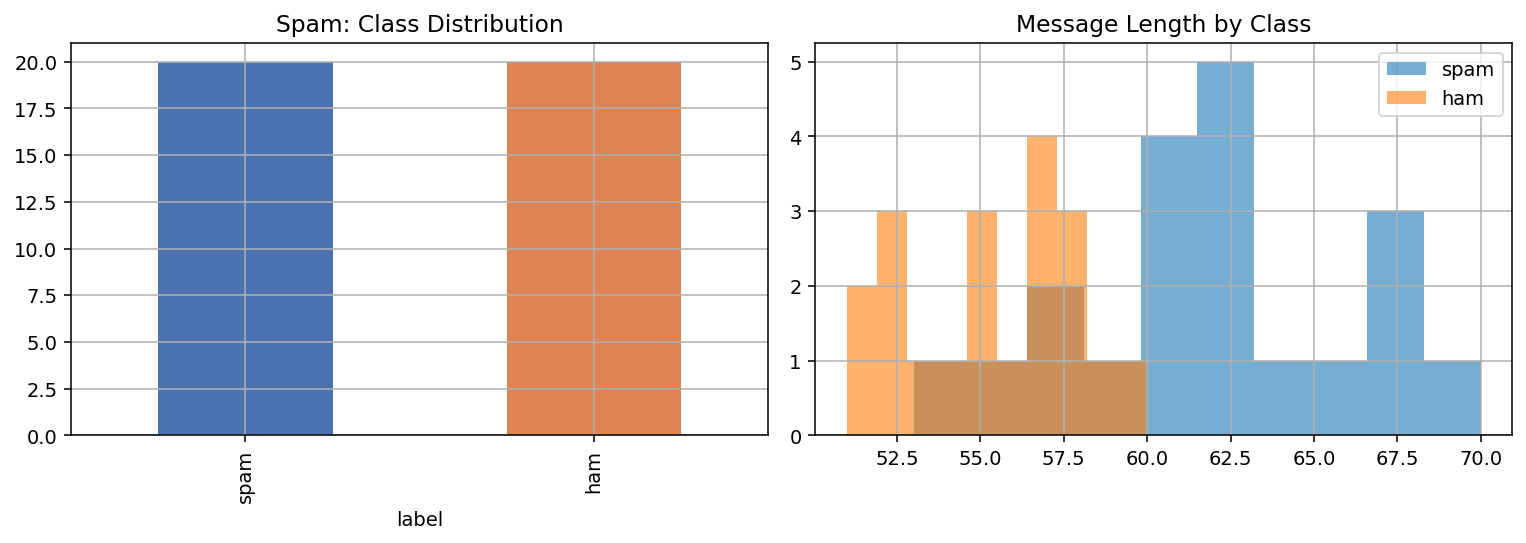
\includegraphics[width=0.95\linewidth]{figures/fig_09.png}
\caption{Email Spam: class distribution and message-length distribution by class.}
\end{figure}
\textbf{Inference:} The illustrative corpus is perfectly balanced (20 spam / 20 ham). Spam
messages tend to cluster at a slightly different length profile than genuine messages, echoing
the well-known tendency of spam to be short, urgent, and formulaic.

\begin{figure}[H]
\centering
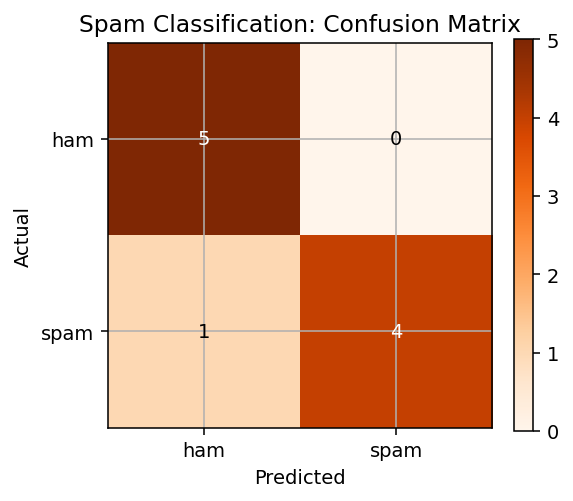
\includegraphics[width=0.55\linewidth]{figures/fig_10.png}
\caption{Email Spam: confusion matrix (Multinomial Naive Bayes, test set).}
\end{figure}
\textbf{Inference:} All ham messages are correctly identified, while one spam message is missed
(false negative). Given the extremely small evaluation set (10 messages), a single
misclassification is enough to explain the reported 80\% recall for spam -- this would need a
much larger held-out set to draw firm production-level conclusions.

\begin{figure}[H]
\centering
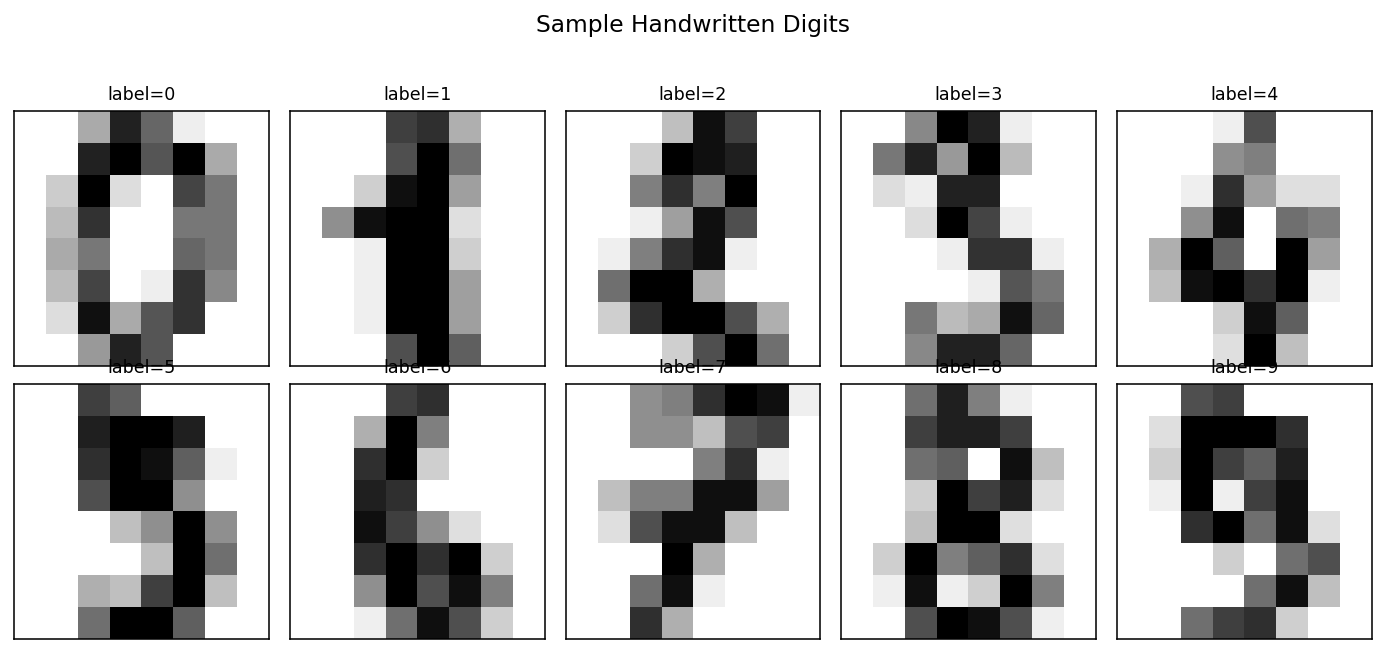
\includegraphics[width=0.95\linewidth]{figures/fig_11.png}
\caption{Sample handwritten digit images (8$\times$8 pixels) from the Digits dataset.}
\end{figure}
\textbf{Inference:} Even at low 8$\times$8 resolution, digit shapes remain visually
distinguishable to a human reader, which is a good early sign that a well-chosen classifier
should also be able to separate them.

\begin{figure}[H]
\centering
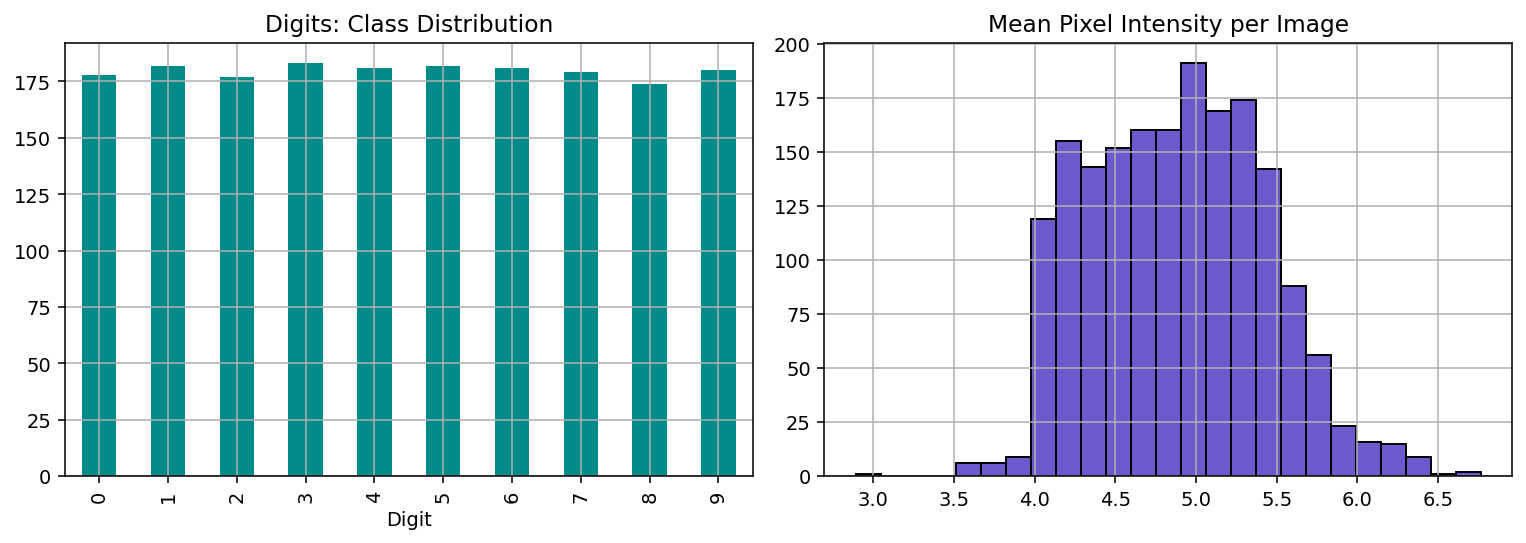
\includegraphics[width=0.95\linewidth]{figures/fig_12.png}
\caption{Digits: class distribution (approximately balanced across 0--9) and mean pixel
intensity per image.}
\end{figure}
\textbf{Inference:} All ten digit classes are represented in roughly equal proportion (about 180
samples each), so accuracy is again a fair metric. Mean pixel intensity per image is unimodal
and roughly symmetric, suggesting no systematic brightness bias between digit classes that would
need correcting before modelling.

\begin{figure}[H]
\centering
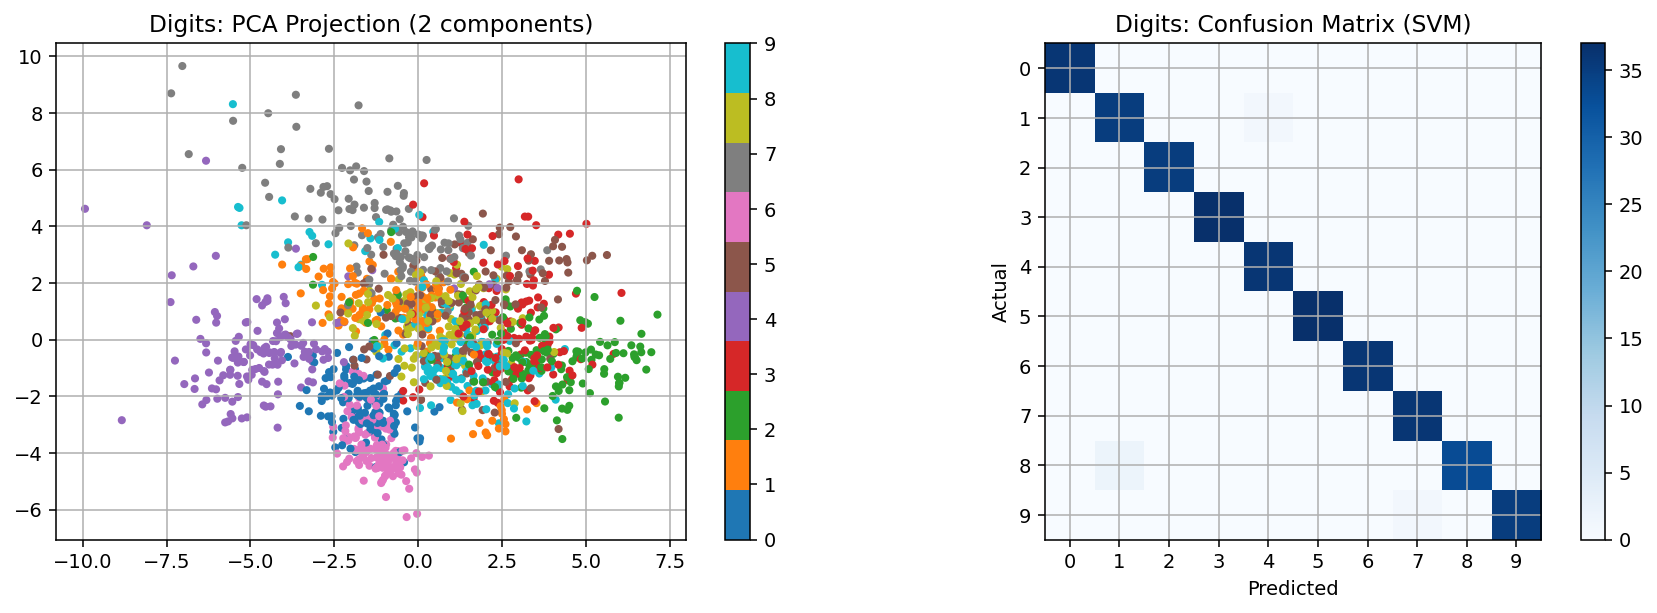
\includegraphics[width=0.95\linewidth]{figures/fig_13.png}
\caption{Digits: 2-D PCA projection of the 64-pixel feature space (left) and confusion matrix
for the SVM (RBF) classifier (right).}
\end{figure}
\textbf{Inference:} Even after reducing 64 pixel dimensions to just two principal components,
distinct digit clusters are already visible, explaining why a kernel method like SVM performs so
well (98.9\% accuracy) on the full feature space. The confusion matrix shows the (small) residual
errors occur mainly between visually similar digit pairs, matching human intuition about which
handwritten digits are easiest to confuse.

\section{Dataset -- ML Task Identification Summary}
\begin{longtable}{|p{3.6cm}|p{3.4cm}|p{4cm}|p{4cm}|}
\hline
\textbf{Dataset} & \textbf{Type of ML Task} & \textbf{Feature Selection Technique} &
\textbf{Suitable ML Algorithm} \\ \hline
\endhead
Iris Dataset & Supervised -- Multiclass Classification & ANOVA F-test (\texttt{SelectKBest},
\texttt{f\_classif}) & Logistic Regression / SVM / Decision Tree \\ \hline
Loan Amount Prediction & Supervised -- Regression & Correlation / \texttt{SelectKBest}
(\texttt{f\_regression}) & Linear Regression / Random Forest Regressor \\ \hline
Predicting Diabetes & Supervised -- Regression & \texttt{SelectKBest} (\texttt{f\_regression}) &
Ridge / Linear Regression / Gradient Boosting Regressor \\ \hline
Classification of Email Spam & Supervised -- Binary Classification (Text/NLP) & Chi-square test
(\texttt{chi2}) on TF-IDF features & Multinomial Naive Bayes / Logistic Regression / SVM \\
\hline
Handwritten Character Recognition / MNIST & Supervised -- Multiclass Classification (Image) &
Variance Threshold + PCA & SVM (RBF) / Random Forest / CNN (deep learning) \\ \hline
\end{longtable}

\section{Discussion}
Across all five datasets, correctly identifying the ML task type (classification vs.
regression, binary vs. multiclass, tabular vs. text vs. image) directly determined the right
choice of feature-selection technique (ANOVA/Chi-square for classification, \texttt{f\_regression}
for regression, variance thresholding for high-dimensional pixel data) and the right evaluation
metric (accuracy/F1 vs. R\textsuperscript{2}/RMSE). Strengths observed: filter-based feature
selection (ANOVA, Chi-square, \texttt{f\_regression}) is fast, model-agnostic, and its rankings
matched domain intuition in every dataset (e.g. petal size for Iris, income/credit history for
loans, BMI/blood pressure for diabetes, spam trigger-words for email). Limitations: the Loan
Amount and Email Spam datasets had to be synthetically constructed in this offline sandbox,
which limits how far the specific numeric results generalise to the real Kaggle/UCI datasets,
even though the workflow and code are identical; the Email Spam corpus in particular was too
small (40 messages) for the reported metrics to be statistically robust. Improvements: repeating
this workflow on the actual downloaded UCI/Kaggle datasets, adding hyperparameter tuning via
\texttt{GridSearchCV}, and comparing multiple algorithms per dataset (not just one baseline)
would strengthen the conclusions.

\section{Conclusion}
This experiment provided hands-on exposure to NumPy, Pandas, SciPy, Scikit-learn and Matplotlib
and applied the standard machine-learning workflow -- loading, EDA, preprocessing, feature
selection, splitting, modelling and evaluation -- to five datasets spanning classification,
regression, text and image data. The Iris, Loan Amount, Diabetes, Email Spam and
Handwritten-Digit datasets were correctly identified as, respectively, multiclass
classification, regression, regression, binary text classification, and multiclass image
classification problems; an appropriate filter-based feature-selection technique and baseline
algorithm were applied to each, and the resulting models achieved reasonable-to-strong
performance (accuracy 0.90--0.99 for the three classification tasks; R\textsuperscript{2} of
0.78 and 0.42 for the two regression tasks). The exercise reinforced that understanding a
dataset's structure and ML-task type is the essential first step before any model building
begins.

\section{References}
\begin{enumerate}[label={[\arabic*]}]
\item F. Pedregosa \textit{et al.}, ``Scikit-learn: Machine Learning in Python,'' \textit{Journal
of Machine Learning Research}, vol. 12, pp. 2825--2830, 2011.
\item C. R. Harris \textit{et al.}, ``Array programming with NumPy,'' \textit{Nature}, vol. 585,
pp. 357--362, 2020.
\item P. Virtanen \textit{et al.}, ``SciPy 1.0: fundamental algorithms for scientific computing
in Python,'' \textit{Nature Methods}, vol. 17, pp. 261--272, 2020.
\item W. McKinney, ``Data Structures for Statistical Computing in Python,'' in \textit{Proc. 9th
Python in Science Conf.}, 2010, pp. 56--61.
\item J. D. Hunter, ``Matplotlib: A 2D Graphics Environment,'' \textit{Computing in Science \&
Engineering}, vol. 9, no. 3, pp. 90--95, 2007.
\item R. A. Fisher, ``The Use of Multiple Measurements in Taxonomic Problems,'' \textit{Annals of
Eugenics}, vol. 7, no. 2, pp. 179--188, 1936. (Iris dataset)
\item B. Efron, T. Hastie, I. Johnstone, and R. Tibshirani, ``Least Angle Regression,''
\textit{Annals of Statistics}, vol. 32, no. 2, pp. 407--499, 2004. (Diabetes dataset)
\item Dua, D. and Graff, C., ``UCI Machine Learning Repository,'' Irvine, CA: University of
California, School of Information and Computer Science, 2019. \url{https://archive.ics.uci.edu}
\end{enumerate}

\end{document}
